\documentclass[8pt]{article}\usepackage[]{graphicx}\usepackage[]{color}
% maxwidth is the original width if it is less than linewidth
% otherwise use linewidth (to make sure the graphics do not exceed the margin)
\makeatletter
\def\maxwidth{ %
  \ifdim\Gin@nat@width>\linewidth
    \linewidth
  \else
    \Gin@nat@width
  \fi
}
\makeatother

\definecolor{fgcolor}{rgb}{0.345, 0.345, 0.345}
\newcommand{\hlnum}[1]{\textcolor[rgb]{0.686,0.059,0.569}{#1}}%
\newcommand{\hlstr}[1]{\textcolor[rgb]{0.192,0.494,0.8}{#1}}%
\newcommand{\hlcom}[1]{\textcolor[rgb]{0.678,0.584,0.686}{\textit{#1}}}%
\newcommand{\hlopt}[1]{\textcolor[rgb]{0,0,0}{#1}}%
\newcommand{\hlstd}[1]{\textcolor[rgb]{0.345,0.345,0.345}{#1}}%
\newcommand{\hlkwa}[1]{\textcolor[rgb]{0.161,0.373,0.58}{\textbf{#1}}}%
\newcommand{\hlkwb}[1]{\textcolor[rgb]{0.69,0.353,0.396}{#1}}%
\newcommand{\hlkwc}[1]{\textcolor[rgb]{0.333,0.667,0.333}{#1}}%
\newcommand{\hlkwd}[1]{\textcolor[rgb]{0.737,0.353,0.396}{\textbf{#1}}}%
\let\hlipl\hlkwb

\usepackage{framed}
\makeatletter
\newenvironment{kframe}{%
 \def\at@end@of@kframe{}%
 \ifinner\ifhmode%
  \def\at@end@of@kframe{\end{minipage}}%
  \begin{minipage}{\columnwidth}%
 \fi\fi%
 \def\FrameCommand##1{\hskip\@totalleftmargin \hskip-\fboxsep
 \colorbox{shadecolor}{##1}\hskip-\fboxsep
     % There is no \\@totalrightmargin, so:
     \hskip-\linewidth \hskip-\@totalleftmargin \hskip\columnwidth}%
 \MakeFramed {\advance\hsize-\width
   \@totalleftmargin\z@ \linewidth\hsize
   \@setminipage}}%
 {\par\unskip\endMakeFramed%
 \at@end@of@kframe}
\makeatother

\definecolor{shadecolor}{rgb}{.97, .97, .97}
\definecolor{messagecolor}{rgb}{0, 0, 0}
\definecolor{warningcolor}{rgb}{1, 0, 1}
\definecolor{errorcolor}{rgb}{1, 0, 0}
\newenvironment{knitrout}{}{} % an empty environment to be redefined in TeX

\usepackage{alltt}
%\usepackage{amsbsy} % for \boldsymbol and \pmb
\usepackage{graphicx} % To include pdf files!
\usepackage{amsmath}
\usepackage{amsbsy, enumitem}
\usepackage{amsfonts,multicol,xcolor}
\usepackage[linesnumbered,ruled,vlined]{algorithm2e}
\usepackage[version=4]{mhchem}
\usepackage[colorlinks=true, pdfstartview=FitV, linkcolor=blue, citecolor=blue, urlcolor=blue]{hyperref} % For links
\newcommand{\highlight}[1]{% 
\colorbox{red!50}{$\displaystyle#1$}}
\newcommand{\matr}[1]{\mathbf{#1}}
\DeclareMathOperator{\E}{E}
\DeclareMathOperator{\var}{var}
\DeclareMathOperator{\cov}{cov}
\DeclareMathOperator{\cor}{cor}
\DeclareMathOperator*{\argmin}{argmin} 
\DeclareMathOperator*{\argmax}{argmax}
\IfFileExists{upquote.sty}{\usepackage{upquote}}{}
\begin{document}
\pagestyle{plain}
\title{Numerical Simulation}
\author{Bowei Xiao}
\date{}
\maketitle
\begin{enumerate}
\item Running the simulation as suggested. See Figure \ref{fig:sim1} as below. With the different choice of the initial growth rate, the population growth rate can either pleateau and stay or die down or flucturate. This also shows how sensitive/chaotic the system is to the growth rate.  
\begin{knitrout}
\definecolor{shadecolor}{rgb}{0.969, 0.969, 0.969}\color{fgcolor}\begin{kframe}
\begin{alltt}
\hlkwd{set.seed}\hlstd{(}\hlnum{1020}\hlstd{)}
\hlstd{x0}\hlkwb{=}\hlnum{0.1}\hlstd{; sim1}\hlkwb{=}\hlkwa{NULL}\hlstd{;}
\hlstd{r1}\hlkwb{=}\hlnum{0.5}\hlstd{; r2}\hlkwb{=}\hlnum{2.8}\hlstd{; r3}\hlkwb{=}\hlnum{3.3}
\hlstd{sim1}\hlkwb{=}\hlkwd{data.frame}\hlstd{(}\hlkwc{t}\hlstd{=}\hlnum{0}\hlstd{,}\hlkwc{r1}\hlstd{=x0,}\hlkwc{r2}\hlstd{=x0,}\hlkwc{r3}\hlstd{=x0,}\hlkwc{stringsAsFactors} \hlstd{= F)}
\hlkwa{for} \hlstd{(i} \hlkwa{in} \hlnum{1}\hlopt{:}\hlnum{50}\hlstd{)\{}
  \hlstd{sim1}\hlkwb{=}\hlkwd{rbind}\hlstd{(sim1,}\hlkwd{data.frame}\hlstd{(}\hlkwc{t}\hlstd{=i,}\hlkwc{r1}\hlstd{=r1}\hlopt{*}\hlstd{sim1}\hlopt{$}\hlstd{r1[i]}\hlopt{*}\hlstd{(}\hlnum{1}\hlopt{-}\hlstd{sim1}\hlopt{$}\hlstd{r1[i]),}
                             \hlkwc{r2}\hlstd{=r2}\hlopt{*}\hlstd{sim1}\hlopt{$}\hlstd{r2[i]}\hlopt{*}\hlstd{(}\hlnum{1}\hlopt{-}\hlstd{sim1}\hlopt{$}\hlstd{r2[i]),}
                             \hlkwc{r3}\hlstd{=r3}\hlopt{*}\hlstd{sim1}\hlopt{$}\hlstd{r3[i]}\hlopt{*}\hlstd{(}\hlnum{1}\hlopt{-}\hlstd{sim1}\hlopt{$}\hlstd{r3[i]),}\hlkwc{stringsAsFactors} \hlstd{= F))}
\hlstd{\}}

\hlkwd{plot}\hlstd{(r1}\hlopt{~}\hlstd{t,}\hlkwc{data}\hlstd{=sim1,}\hlkwc{type}\hlstd{=}\hlstr{'l'}\hlstd{,}\hlkwc{col}\hlstd{=}\hlstr{'red'}\hlstd{,}\hlkwc{ylim}\hlstd{=}\hlkwd{c}\hlstd{(}\hlnum{0}\hlstd{,}\hlnum{1}\hlstd{),}\hlkwc{xlab}\hlstd{=}\hlstr{'generations'}\hlstd{,}\hlkwc{ylab}\hlstd{=}\hlstr{'Xn'}\hlstd{)}
\hlkwd{lines}\hlstd{(sim1}\hlopt{$}\hlstd{t,sim1}\hlopt{$}\hlstd{r2,}\hlkwc{col}\hlstd{=}\hlstr{'blue'}\hlstd{)}
\hlkwd{lines}\hlstd{(sim1}\hlopt{$}\hlstd{t,sim1}\hlopt{$}\hlstd{r3,}\hlkwc{col}\hlstd{=}\hlstr{'black'}\hlstd{)}
\hlkwd{legend}\hlstd{(}\hlstr{'topleft'}\hlstd{,}\hlkwc{legend}\hlstd{=}\hlkwd{c}\hlstd{(}\hlstr{'r=0.5'}\hlstd{,}\hlstr{'r=2.8'}\hlstd{,}\hlstr{'r=3.3'}\hlstd{),}
        \hlkwc{col}\hlstd{=}\hlkwd{c}\hlstd{(}\hlstr{'red'}\hlstd{,}\hlstr{'blue'}\hlstd{,}\hlstr{'black'}\hlstd{),}\hlkwc{lty}\hlstd{=}\hlnum{1}\hlstd{,}\hlkwc{cex}\hlstd{=}\hlnum{0.8}\hlstd{)}
\end{alltt}
\end{kframe}\begin{figure}
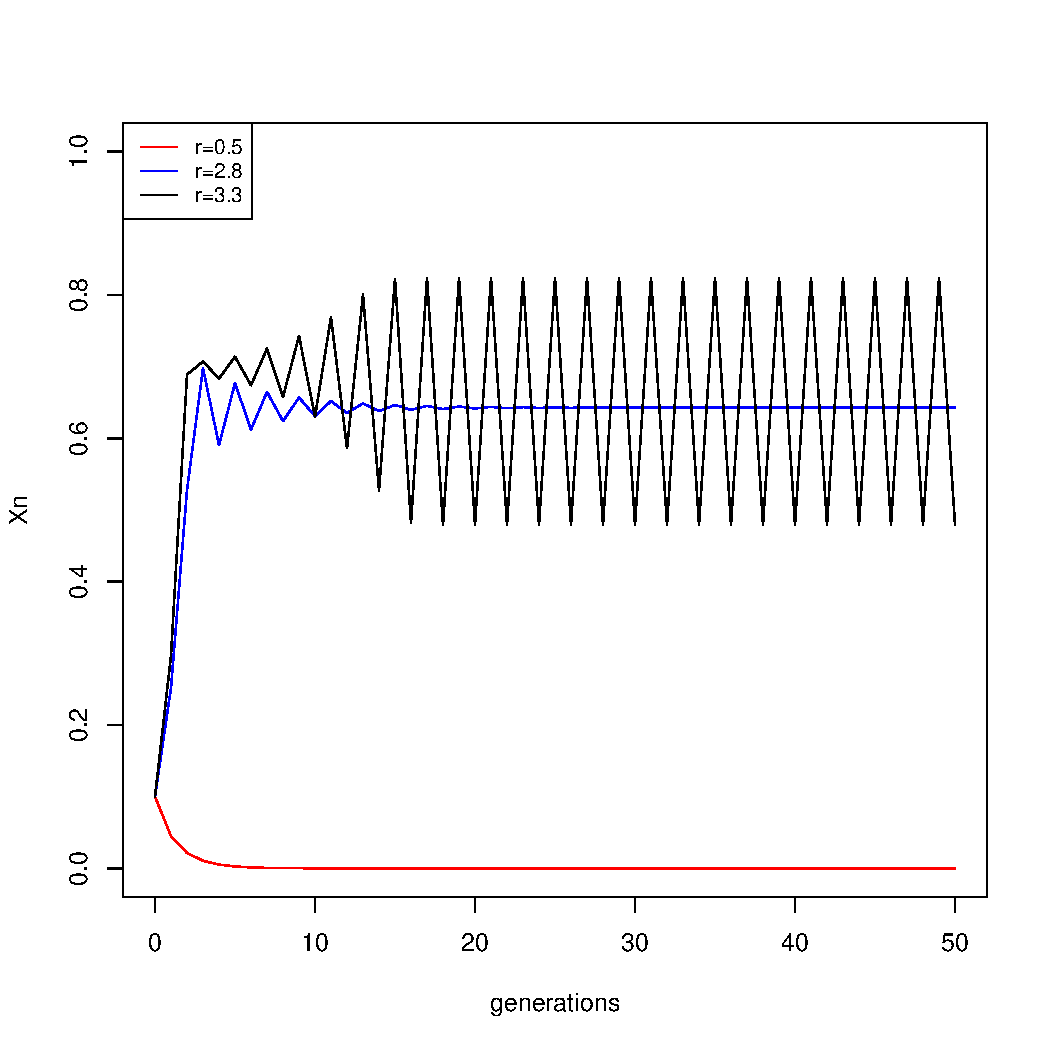
\includegraphics[width=0.9\textwidth]{figure/sim1-1} \caption[population growth with different r]{population growth with different r}\label{fig:sim1}
\end{figure}


\end{knitrout}

\item Coding for Euler method here:
\begin{knitrout}
\definecolor{shadecolor}{rgb}{0.969, 0.969, 0.969}\color{fgcolor}\begin{kframe}
\begin{alltt}
\hlstd{euler_for}\hlkwb{=}\hlkwa{function}\hlstd{(}\hlkwc{x0}\hlstd{,}\hlkwc{t}\hlstd{,}\hlkwc{h}\hlstd{)\{}
  \hlstd{step}\hlkwb{=}\hlkwd{data.frame}\hlstd{(}\hlkwc{x}\hlstd{=x0,}\hlkwc{t}\hlstd{=}\hlnum{0}\hlstd{); tmax}\hlkwb{=}\hlkwd{as.integer}\hlstd{(t}\hlopt{/}\hlstd{h}\hlopt{+}\hlnum{0.5}\hlstd{)}
  \hlkwa{for} \hlstd{(i} \hlkwa{in} \hlnum{1}\hlopt{:}\hlstd{tmax)\{}
    \hlstd{step}\hlkwb{=}\hlkwd{rbind}\hlstd{(step,}\hlkwd{data.frame}\hlstd{(}\hlkwc{x}\hlstd{=step}\hlopt{$}\hlstd{x[i]}\hlopt{+}\hlstd{h}\hlopt{*}\hlstd{step}\hlopt{$}\hlstd{x[i],}\hlkwc{t}\hlstd{=h}\hlopt{*}\hlstd{i))}
  \hlstd{\}}
  \hlkwd{return}\hlstd{(step)}
\hlstd{\}}
\hlstd{sol1}\hlkwb{=}\hlkwd{euler_for}\hlstd{(}\hlkwc{x0}\hlstd{=}\hlnum{1}\hlstd{,}\hlkwc{t}\hlstd{=}\hlnum{5}\hlstd{,}\hlkwc{h}\hlstd{=}\hlnum{0.1}\hlstd{);}
\hlstd{sol2}\hlkwb{=}\hlkwd{euler_for}\hlstd{(}\hlkwc{x0}\hlstd{=}\hlnum{1}\hlstd{,}\hlkwc{t}\hlstd{=}\hlnum{5}\hlstd{,}\hlkwc{h}\hlstd{=}\hlnum{0.01}\hlstd{);}
\hlstd{sol3}\hlkwb{=}\hlkwd{euler_for}\hlstd{(}\hlkwc{x0}\hlstd{=}\hlnum{1}\hlstd{,}\hlkwc{t}\hlstd{=}\hlnum{5}\hlstd{,}\hlkwc{h}\hlstd{=}\hlnum{0.001}\hlstd{);}

\hlkwd{plot}\hlstd{(}\hlkwd{seq}\hlstd{(}\hlnum{0}\hlstd{,}\hlnum{5}\hlstd{,}\hlnum{0.001}\hlstd{),}\hlkwd{exp}\hlstd{(}\hlkwd{seq}\hlstd{(}\hlnum{0}\hlstd{,}\hlnum{5}\hlstd{,}\hlnum{0.001}\hlstd{)),}\hlkwc{type}\hlstd{=}\hlstr{'l'}\hlstd{,}\hlkwc{col}\hlstd{=}\hlstr{'red'}\hlstd{,}\hlkwc{lwd}\hlstd{=}\hlnum{2}\hlstd{)}
\hlkwd{lines}\hlstd{(sol1}\hlopt{$}\hlstd{t,sol1}\hlopt{$}\hlstd{x,}\hlkwc{col}\hlstd{=}\hlstr{'blue'}\hlstd{,}\hlkwc{lty}\hlstd{=}\hlnum{1}\hlstd{)}
\hlkwd{lines}\hlstd{(sol2}\hlopt{$}\hlstd{t,sol2}\hlopt{$}\hlstd{x,}\hlkwc{col}\hlstd{=}\hlstr{'blue'}\hlstd{,}\hlkwc{lty}\hlstd{=}\hlnum{2}\hlstd{)}
\hlkwd{lines}\hlstd{(sol3}\hlopt{$}\hlstd{t,sol3}\hlopt{$}\hlstd{x,}\hlkwc{col}\hlstd{=}\hlstr{'blue'}\hlstd{,}\hlkwc{lty}\hlstd{=}\hlnum{5}\hlstd{)}
\hlkwd{legend}\hlstd{(}\hlstr{'topleft'}\hlstd{,}\hlkwc{legend}\hlstd{=}\hlkwd{c}\hlstd{(}\hlstr{'step=0.1'}\hlstd{,}\hlstr{'step=0.01'}\hlstd{,}\hlstr{'step=0.001'}\hlstd{,}\hlstr{'y=exp(x)'}\hlstd{),}
        \hlkwc{col}\hlstd{=}\hlkwd{c}\hlstd{(}\hlkwd{rep}\hlstd{(}\hlstr{'blue'}\hlstd{,}\hlnum{3}\hlstd{),}\hlstr{'red'}\hlstd{),}\hlkwc{lty}\hlstd{=}\hlkwd{c}\hlstd{(}\hlnum{1}\hlstd{,}\hlnum{2}\hlstd{,}\hlnum{5}\hlstd{,}\hlnum{1}\hlstd{),}\hlkwc{cex}\hlstd{=}\hlnum{0.8}\hlstd{)}
\end{alltt}
\end{kframe}\begin{figure}
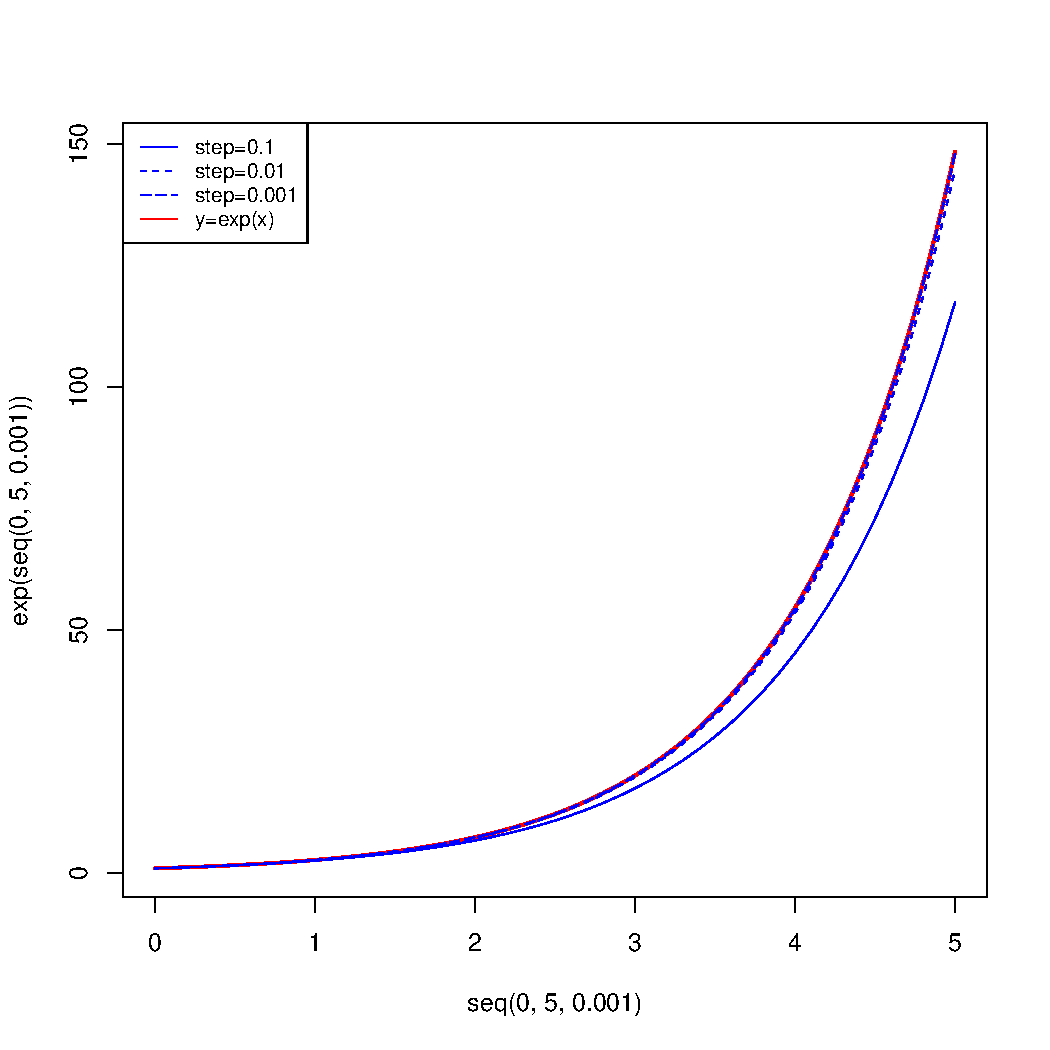
\includegraphics[width=0.9\textwidth]{figure/euler-1} \caption[solution wrt h]{solution wrt h}\label{fig:euler}
\end{figure}


\end{knitrout}
All solutions calculated using such algorithm is close to $y=exp(x)$. Of course, the smaller the step is, the closer the numerical values approaches to the real analytical solutioon.

\item FitzHugh-Nagumo model:\\
\begin{knitrout}
\definecolor{shadecolor}{rgb}{0.969, 0.969, 0.969}\color{fgcolor}\begin{kframe}
\begin{alltt}
\hlstd{fhn}\hlkwb{=}\hlkwa{function}\hlstd{(}\hlkwc{t}\hlstd{,}\hlkwc{v0}\hlstd{,}\hlkwc{w0}\hlstd{,}\hlkwc{I}\hlstd{,}\hlkwc{h}\hlstd{=}\hlnum{0.01}\hlstd{)\{}
  \hlstd{tmax}\hlkwb{=}\hlkwd{as.integer}\hlstd{(t}\hlopt{/}\hlstd{h}\hlopt{+}\hlnum{0.5}\hlstd{); a}\hlkwb{=}\hlnum{0.7}\hlstd{;b}\hlkwb{=}\hlnum{0.8}\hlstd{;eps}\hlkwb{=}\hlnum{0.08}\hlstd{;}
  \hlstd{step}\hlkwb{=}\hlkwd{data.frame}\hlstd{(}\hlkwc{v}\hlstd{=v0,}\hlkwc{w}\hlstd{=w0,}\hlkwc{t}\hlstd{=}\hlnum{0}\hlstd{); tmax}\hlkwb{=}\hlkwd{as.integer}\hlstd{(t}\hlopt{/}\hlstd{h}\hlopt{+}\hlnum{0.5}\hlstd{)}
  \hlkwa{for} \hlstd{(i} \hlkwa{in} \hlnum{1}\hlopt{:}\hlstd{tmax)\{}
    \hlstd{vi}\hlkwb{=}\hlstd{step}\hlopt{$}\hlstd{v[i]; wi}\hlkwb{=}\hlstd{step}\hlopt{$}\hlstd{w[i];}
    \hlstd{step}\hlkwb{=}\hlkwd{rbind}\hlstd{(step,}\hlkwd{data.frame}\hlstd{(}\hlkwc{v}\hlstd{=vi}\hlopt{+}\hlstd{h}\hlopt{*}\hlstd{(vi}\hlopt{-}\hlstd{vi}\hlopt{^}\hlnum{3}\hlopt{/}\hlnum{3}\hlopt{-}\hlstd{wi}\hlopt{+}\hlstd{I),}
                               \hlkwc{w}\hlstd{=wi}\hlopt{+}\hlstd{h}\hlopt{*}\hlstd{(eps}\hlopt{*}\hlstd{(vi}\hlopt{+}\hlstd{a}\hlopt{-}\hlstd{b}\hlopt{*}\hlstd{wi)),}\hlkwc{t}\hlstd{=h}\hlopt{*}\hlstd{i))}
  \hlstd{\}}
  \hlkwd{return}\hlstd{(step)}
\hlstd{\}}
\hlstd{sol1}\hlkwb{=}\hlkwd{fhn}\hlstd{(}\hlkwc{t}\hlstd{=}\hlnum{400}\hlstd{,}\hlkwc{v0}\hlstd{=}\hlnum{1}\hlstd{,}\hlkwc{w0}\hlstd{=}\hlnum{0.1}\hlstd{,}\hlkwc{I}\hlstd{=}\hlnum{0.5}\hlstd{)}
\hlkwd{plot}\hlstd{(v}\hlopt{~}\hlstd{t,sol1,}\hlkwc{type}\hlstd{=}\hlstr{'l'}\hlstd{)}
\end{alltt}
\end{kframe}\begin{figure}
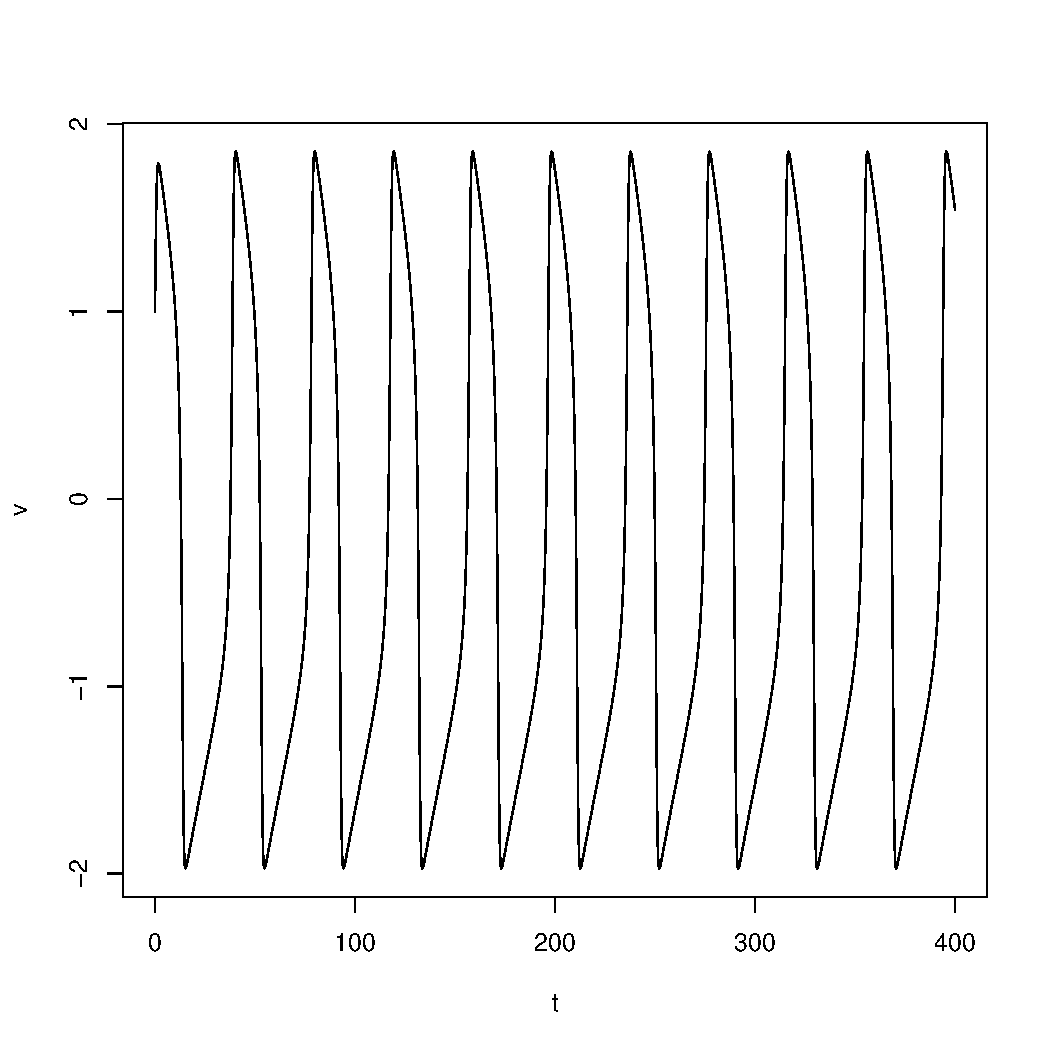
\includegraphics[width=0.9\textwidth]{figure/fhn1-1} \caption[v-t plot]{v-t plot}\label{fig:fhn1}
\end{figure}


\end{knitrout}
From Figure \ref{fig:fhn1}, clearly there is osciallations.\\
Now look at $v$ vs $w$ with the v-nullcline (in blue) and w-nullcline (in red); See Figure \ref{fig:fhn2}\\
\begin{knitrout}
\definecolor{shadecolor}{rgb}{0.969, 0.969, 0.969}\color{fgcolor}\begin{kframe}
\begin{alltt}
\hlkwd{plot}\hlstd{(w}\hlopt{~}\hlstd{v,sol1,}\hlkwc{type}\hlstd{=}\hlstr{'l'}\hlstd{)}
\hlcom{#nullcline}
\hlcom{#w-line: v+a-bw=0 -> w=1/b*V+a/b}
\hlcom{#v-line v-v^3/3-w+I=0 -> w=-1/3v^3+V+I}
\hlkwd{lines}\hlstd{(sol1}\hlopt{$}\hlstd{v,(sol1}\hlopt{$}\hlstd{v}\hlopt{+}\hlnum{0.7}\hlstd{)}\hlopt{/}\hlnum{0.8}\hlstd{,}\hlkwc{col}\hlstd{=}\hlstr{'red'}\hlstd{)}
\hlkwd{lines}\hlstd{(sol1}\hlopt{$}\hlstd{v,}\hlopt{-}\hlnum{1}\hlopt{/}\hlnum{3}\hlopt{*}\hlstd{sol1}\hlopt{$}\hlstd{v}\hlopt{**}\hlnum{3}\hlopt{+}\hlstd{sol1}\hlopt{$}\hlstd{v}\hlopt{+}\hlnum{0.5}\hlstd{,}\hlkwc{col}\hlstd{=}\hlstr{'blue'}\hlstd{)}
\end{alltt}
\end{kframe}\begin{figure}
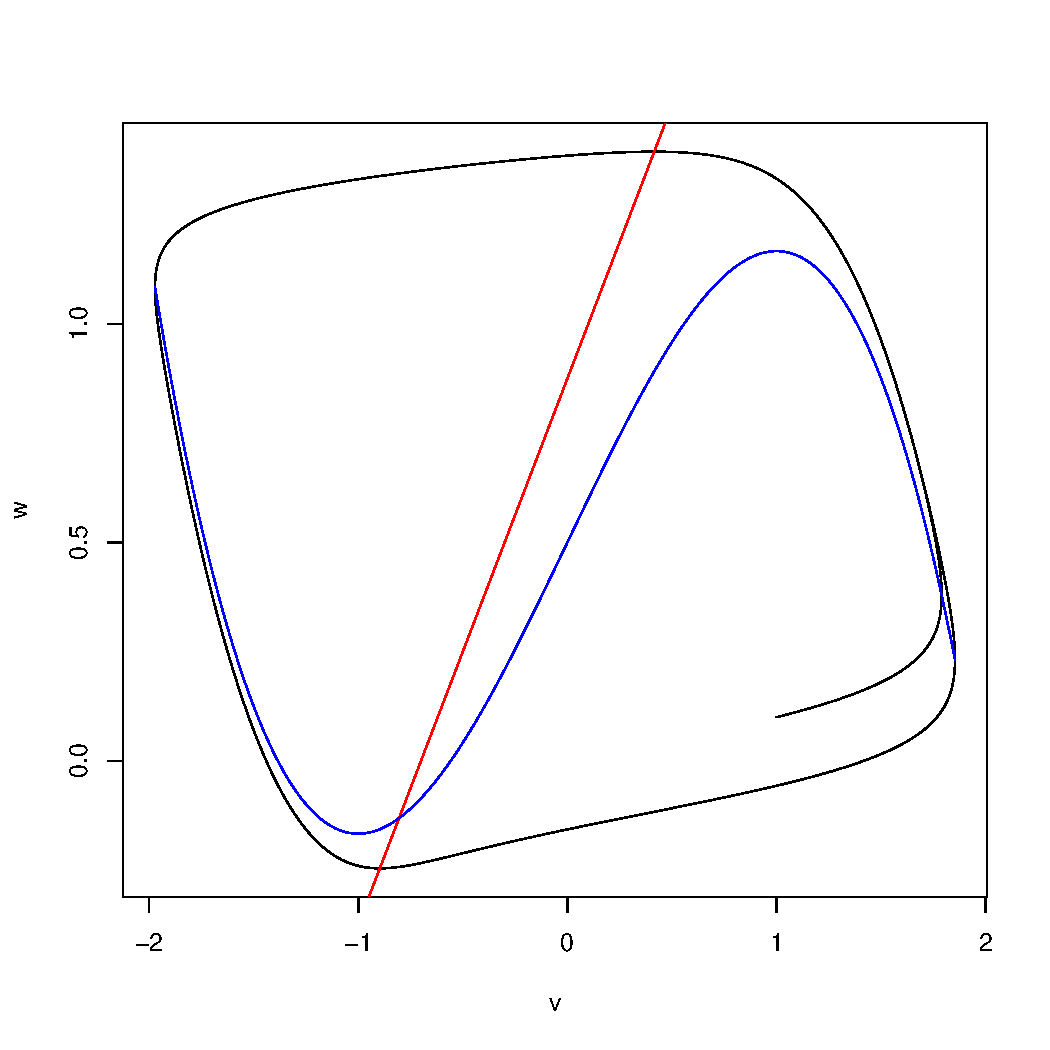
\includegraphics[width=0.9\textwidth]{figure/fhn2-1} \caption[w-v plot]{w-v plot}\label{fig:fhn2}
\end{figure}


\end{knitrout}
We clearly see the loop pattern.\\
To calculate fix point. We solved for 
\begin{eqnarray*}
v-v^3/3-w+I&=&0\\
\epsilon (v+a-bw)&=&0
\end{eqnarray*}
This solves for $v*$, and we can calculate the Jacobians as :\\
\begin{pmatrix}
1-$v^2$ & -1 \\
$\epsilon$ & $-b*\epsilon$ 
\end{pmatrix}
Thus, a eigendecomposition at fixed point $v*$ will look at this:\\
\begin{knitrout}
\definecolor{shadecolor}{rgb}{0.969, 0.969, 0.969}\color{fgcolor}\begin{kframe}
\begin{alltt}
\hlstd{a}\hlkwb{=}\hlnum{0.7}\hlstd{;b}\hlkwb{=}\hlnum{0.8}\hlstd{; I}\hlkwb{=}\hlnum{0.5}\hlstd{;eps}\hlkwb{=}\hlnum{0.08}\hlstd{;}
\hlcom{#-(v+a)/b+I+v-1/3v^3=0 -> (-a/b+I)+(1-1/b)v-1/3v^3=0}
\hlstd{vp}\hlkwb{=}\hlkwd{polyroot}\hlstd{(}\hlkwd{c}\hlstd{(}\hlopt{-}\hlstd{a}\hlopt{/}\hlstd{b}\hlopt{+}\hlstd{I,}\hlnum{1}\hlopt{-}\hlnum{1}\hlopt{/}\hlstd{b,}\hlnum{0}\hlstd{,}\hlopt{-}\hlnum{1}\hlopt{/}\hlnum{3}\hlstd{));}
\hlstd{vp}
\end{alltt}
\begin{verbatim}
## [1]  0.4024239+1.111681i -0.8048477-0.000000i  0.4024239-1.111681i
\end{verbatim}
\begin{alltt}
\hlcom{# take the real-value one as v*}
\hlkwd{eigen}\hlstd{(}\hlkwd{matrix}\hlstd{(}\hlkwd{c}\hlstd{(}\hlnum{1}\hlopt{-}\hlstd{vp[}\hlnum{2}\hlstd{]}\hlopt{^}\hlnum{2}\hlstd{,}\hlopt{-}\hlnum{1}\hlstd{,eps,}\hlopt{-}\hlstd{b}\hlopt{*}\hlstd{eps),}\hlnum{2}\hlstd{,}\hlnum{2}\hlstd{))}
\end{alltt}
\begin{verbatim}
## eigen() decomposition
## $values
## [1] 0.1441101-0.1915469i 0.1441101+0.1915469i
## 
## $vectors
##                       [,1]                  [,2]
## [1,] -0.2002540+0.1843161i -0.2002540-0.1843161i
## [2,]  0.9622504+0.0000000i  0.9622504+0.0000000i
\end{verbatim}
\end{kframe}
\end{knitrout}

We observed positive real parts for both of the eigenvalues. This is expected because we see from the phase-plane plot that the direction is not stable.\\
Now, calculate again with $I=0$. We can see the negative eigenvalues, indicating a stable focues.\\
\begin{knitrout}
\definecolor{shadecolor}{rgb}{0.969, 0.969, 0.969}\color{fgcolor}\begin{kframe}
\begin{alltt}
\hlstd{a}\hlkwb{=}\hlnum{0.7}\hlstd{;b}\hlkwb{=}\hlnum{0.8}\hlstd{; I}\hlkwb{=}\hlnum{0}\hlstd{;eps}\hlkwb{=}\hlnum{0.08}\hlstd{;}
\hlcom{#-(v+a)/b+I+v-1/3v^3=0 -> (-a/b+I)+(1-1/b)v-1/3v^3=0}
\hlstd{vp}\hlkwb{=}\hlkwd{polyroot}\hlstd{(}\hlkwd{c}\hlstd{(}\hlopt{-}\hlstd{a}\hlopt{/}\hlstd{b}\hlopt{+}\hlstd{I,}\hlnum{1}\hlopt{-}\hlnum{1}\hlopt{/}\hlstd{b,}\hlnum{0}\hlstd{,}\hlopt{-}\hlnum{1}\hlopt{/}\hlnum{3}\hlstd{));}
\hlstd{vp}
\end{alltt}
\begin{verbatim}
## [1]  0.599704+1.352381i -1.199408+0.000000i  0.599704-1.352381i
\end{verbatim}
\begin{alltt}
\hlcom{# take the real-value one as v*}
\hlkwd{eigen}\hlstd{(}\hlkwd{matrix}\hlstd{(}\hlkwd{c}\hlstd{(}\hlnum{1}\hlopt{-}\hlstd{vp[}\hlnum{2}\hlstd{]}\hlopt{^}\hlnum{2}\hlstd{,}\hlopt{-}\hlnum{1}\hlstd{,eps,}\hlopt{-}\hlstd{b}\hlopt{*}\hlstd{eps),}\hlnum{2}\hlstd{,}\hlnum{2}\hlstd{))}
\end{alltt}
\begin{verbatim}
## eigen() decomposition
## $values
## [1] -0.2512898+0.2119493i -0.2512898-0.2119493i
## 
## $vectors
##                      [,1]                 [,2]
## [1,] 0.1802197-0.2039484i 0.1802197+0.2039484i
## [2,] 0.9622504+0.0000000i 0.9622504+0.0000000i
\end{verbatim}
\end{kframe}
\end{knitrout}
Now, ranging $I$ from 0 to 0.5, and recreate the bifurcation diagram as in Figure \ref{fig:sol3}.\\
\begin{knitrout}
\definecolor{shadecolor}{rgb}{0.969, 0.969, 0.969}\color{fgcolor}\begin{kframe}
\begin{alltt}
\hlstd{h}\hlkwb{=}\hlnum{0.01}\hlstd{; I}\hlkwb{=}\hlnum{0.5}\hlstd{; tmax}\hlkwb{=}\hlkwd{as.integer}\hlstd{(}\hlnum{0.5}\hlopt{/}\hlstd{h}\hlopt{+}\hlnum{0.5}\hlstd{)}
\hlstd{a}\hlkwb{=}\hlnum{0.7}\hlstd{;b}\hlkwb{=}\hlnum{0.8}\hlstd{;eps}\hlkwb{=}\hlnum{0.08}\hlstd{;}
\hlcom{#when I=0, iot is stable}
\hlstd{sim3}\hlkwb{=}\hlkwd{data.frame}\hlstd{(}\hlkwc{I}\hlstd{=}\hlnum{0}\hlstd{,}\hlkwc{v}\hlstd{=vp[}\hlnum{2}\hlstd{],}\hlkwc{stable}\hlstd{=}\hlnum{1}\hlstd{)}
\hlkwa{for} \hlstd{(i} \hlkwa{in} \hlnum{1}\hlopt{:}\hlstd{tmax)\{}
  \hlstd{I}\hlkwb{=}\hlstd{i}\hlopt{*}\hlstd{h}
  \hlstd{vp}\hlkwb{=}\hlkwd{polyroot}\hlstd{(}\hlkwd{c}\hlstd{(}\hlopt{-}\hlstd{a}\hlopt{/}\hlstd{b}\hlopt{+}\hlstd{I,}\hlnum{1}\hlopt{-}\hlnum{1}\hlopt{/}\hlstd{b,}\hlnum{0}\hlstd{,}\hlopt{-}\hlnum{1}\hlopt{/}\hlnum{3}\hlstd{))}
  \hlcom{#find the real-valued v*; tolerance 1e-10}
  \hlstd{vn}\hlkwb{=}\hlstd{vp[}\hlkwd{which}\hlstd{(}\hlkwd{abs}\hlstd{(}\hlkwd{Im}\hlstd{(vp))}\hlopt{<}\hlnum{1e-10}\hlstd{)]}
  \hlstd{evals}\hlkwb{=}\hlkwd{eigen}\hlstd{(}\hlkwd{matrix}\hlstd{(}\hlkwd{c}\hlstd{(}\hlnum{1}\hlopt{-}\hlstd{vn}\hlopt{^}\hlnum{2}\hlstd{,}\hlopt{-}\hlnum{1}\hlstd{,eps,}\hlopt{-}\hlstd{b}\hlopt{*}\hlstd{eps),}\hlnum{2}\hlstd{,}\hlnum{2}\hlstd{))}\hlopt{$}\hlstd{values}
  \hlcom{# if real part of eigevalue is positive -> unstable(0); negative stable(1)}
  \hlstd{sim3}\hlkwb{=}\hlkwd{rbind}\hlstd{(sim3,}\hlkwd{data.frame}\hlstd{(}\hlkwc{I}\hlstd{=I,}\hlkwc{v}\hlstd{=vn,}
                   \hlkwc{stable}\hlstd{=}\hlkwd{as.numeric}\hlstd{(}\hlkwd{sum}\hlstd{(}\hlkwd{Re}\hlstd{(evals)}\hlopt{<}\hlnum{0}\hlstd{)}\hlopt{==}\hlnum{2}\hlstd{)))}
\hlstd{\}}
\hlcom{#create bifurcation diagram}
\hlkwd{plot}\hlstd{(sim3}\hlopt{$}\hlstd{I,sim3}\hlopt{$}\hlstd{v,}\hlkwc{col}\hlstd{=}\hlkwd{c}\hlstd{(}\hlstr{'red'}\hlstd{,}\hlstr{'blue'}\hlstd{)[sim3}\hlopt{$}\hlstd{stable}\hlopt{+}\hlnum{1}\hlstd{])}
\end{alltt}


{\ttfamily\noindent\color{warningcolor}{\#\# Warning in xy.coords(x, y, xlabel, ylabel, log): imaginary parts discarded in coercion}}\end{kframe}\begin{figure}
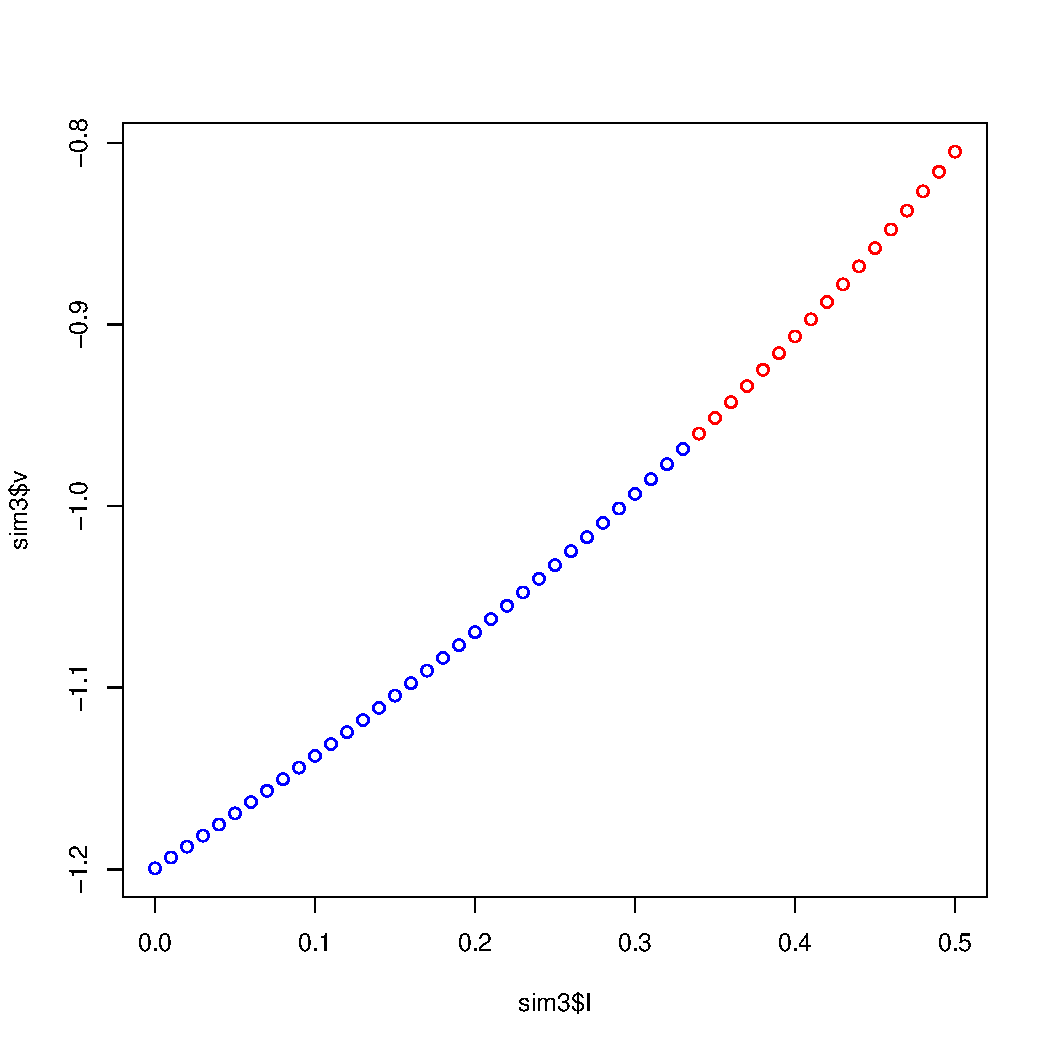
\includegraphics[width=0.9\textwidth]{figure/sol3-1} \caption[w-v plot]{w-v plot}\label{fig:sol3}
\end{figure}


\end{knitrout}
\end{enumerate}
\end{document}
